\section{Risoluzione del problema}\label{sec:qiskit}

Per simulare il problema di ottimizzazione del portafoglio, 
abbiamo utilizzato un approccio basato su un modello generativo 
per produrre dati storici. La generazione dei dati è stata 
realizzata tramite una classe fornita da Qiskit, \texttt{RandomDataProvider}, 
che, a partire da parametri come il numero di asset, il 
periodo temporale e un seme per la riproducibilità, ha 
prodotto una tabella di valori rappresentante l'andamento dei 
prezzi degli asset nel tempo (Tabella~\ref{tab:dati-tickers}). 
Inoltre, per rendere più intuitiva la visualizzazione dei dati, 
abbiamo sviluppato uno script che crea un grafico per ciascun asset, 
rappresentando l'andamento temporale dei prezzi (Figura~\ref{fig:graficiAssets}).

\begin{table}[h]
    \centering
    \renewcommand{\arraystretch}{1.5}
    \begin{tabular}{|c|c|c|c|c|}
    \hline
    \textbf{Data} & \textbf{Ticker\_0} & \textbf{Ticker\_1} & \textbf{Ticker\_2} & \textbf{Ticker\_3} \\
    \hline
    2016--01--01 & 80.0573 & 38.8648 & 69.2682 & 76.1653 \\
    \hline
    2016--01--02 & 80.3390 & 38.7966 & 69.5354 & 76.6583 \\
    \hline
    2016--01--03 & 79.4722 & 39.0100 & 70.7954 & 76.0500 \\
    \hline
    \ldots & \ldots & \ldots & \ldots & \ldots \\
    \hline
    \end{tabular}
    \caption{Esempio di dati generati dalla classe \texttt{RandomDataProvider} 
        con un numero di asset uguale a 4 e un periodo temporale che parte dal 01/01/2016.}
    \label{tab:dati-tickers}
\end{table}

Successivamente, sono stati calcolati i rendimenti medi per ciascun asset 
(Formula~\ref{eqn:matriceRendimentiAttesi}) e la matrice di covarianza 
(Formula~\ref{eqn:matriceCovarianza}) utilizzando i metodi offerti dalla 
classe \texttt{RandomDataProvider}. Questi due elementi rappresentano una 
componente fondamentale per la PO, in quanto i 
rendimenti medi forniscono una misura dell'aspettativa di guadagno, mentre 
la matrice di covarianza descrive la relazione tra le variazioni dei prezzi 
dei diversi asset.

\begin{lstlisting}[language=python, caption={Calcolo dei rendimenti attesi e della matrice di covarianza.}]
 mu = data_provider.get_period_return_mean_vector()
 sigma = data_provider.get_period_return_covariance_matrix()
\end{lstlisting}

Per favorire una migliore comprensione e visualizzazione della matrice di 
covarianza, ne è stato generato un grafico (Figura~\ref{fig:matriceCovarianza}): 
questo consente di evidenziare visivamente le correlazioni tra i diversi asset.

\begin{figure}[h!]
    \centering
    \begin{subfigure}{0.52\textwidth}
        \centering
        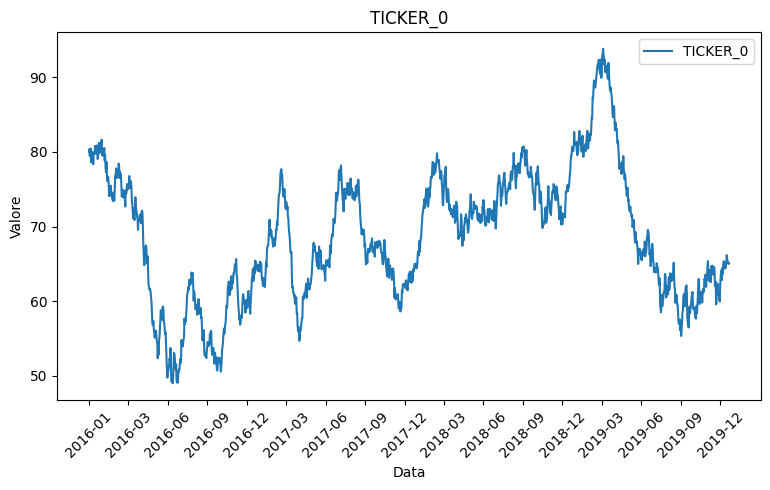
\includegraphics[width=\textwidth]{images/graficoAsset.png}
        \caption{Andamento temporale di un asset.}
        \label{fig:graficiAssets}
    \end{subfigure}
    \hfill
    \begin{subfigure}{0.45\textwidth}
        \centering
        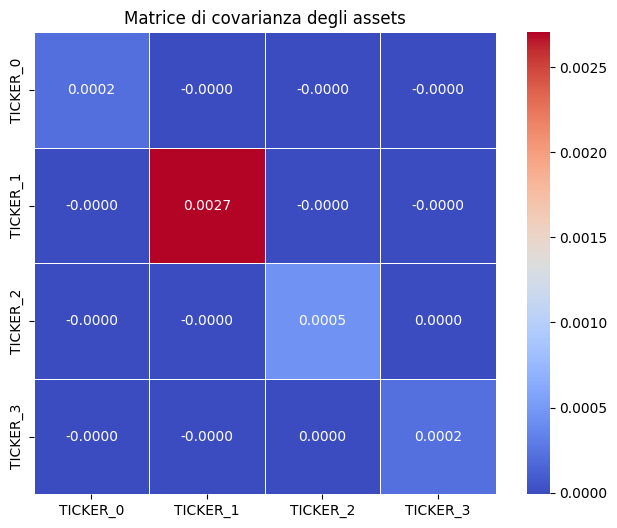
\includegraphics[width=\textwidth]{images/matriceCovarianza.png}
        \caption{Esempio di matrice di covarianza.\footnotemark}
        \label{fig:matriceCovarianza}
    \end{subfigure}
    \caption{(a) Andamento dei prezzi degli asset generati, e (b) matrice di covarianza calcolata.}
    %\label{fig:}
\end{figure}

\footnotetext{I valori della matrice sono stati moltiplicati per $10^5$ per facilitare la lettura nella relazione, mentre per i calcoli sono stati utilizzati i valori originali.}

Dopo aver calcolato i rendimenti medi e la matrice di covarianza per ciascun 
asset, procediamo con la configurazione del problema di ottimizzazione. 
Il fattore di rischio viene impostato a \textit{0.2}, permettendo di bilanciare il 
trade-off tra rendimento e rischio del portafoglio. Il budget viene definito come 
i due terzi del numero totale di asset (\texttt{assets / 3 * 2}). Viene inoltre 
definita la penalità (\texttt{penalty}) uguale al valore del budget per gestire la 
violazione dei vincoli.

Il problema viene quindi configurato attraverso l'inizializzazione di 
un'istanza della classe \texttt{PortfolioOptimization}, alla quale vengono 
passati i parametri fondamentali: il vettore dei rendimenti attesi 
(\texttt{expected\_returns}), la matrice di covarianza (\texttt{covariances}), 
il fattore di rischio (\texttt{risk\_factor}) e il budget (\texttt{budget}). 
La configurazione finale produce 
un output che specifica il numero totale di asset disponibili, 
il budget allocato, la penalità impostata e il fattore di rischio 
utilizzato. Il problema viene infine convertito in un programma 
quadratico attraverso il metodo \texttt{to\_quadratic\_program} per la 
successiva ottimizzazione.

\begin{lstlisting}[language=python, caption={Configurazione del problema di PO.}]
 risk_factor = 0.2
 budget = int(assets / 3 * 2)
 penalty = budget

 po = PortfolioOptimization(
     expected_returns=mu, 
     covariances=sigma, 
     risk_factor=risk_factor, 
     budget=budget
 )
 qp = po.to_quadratic_program()
\end{lstlisting}

\paragraph{Risoluzione classica del problema}
Per ottenere una soluzione di riferimento al nostro problema di ottimizzazione, 
utilizziamo un approccio classico basato su autovalori. In particolare, 
impieghiamo il risolutore \texttt{NumPyMinimumEigensolver}, un algoritmo 
che calcola in modo esatto gli autovalori del problema. Questo risolutore 
viene integrato attraverso \texttt{MinimumEigenOptimizer}, un wrapper  
che fornisce un'interfaccia conveniente per utilizzare il solver e
risolvere il problema di ottimizzazione.

\begin{lstlisting}[language=python, caption={Risoluzione classica del problema utilizzando \texttt{NumPyMinimumEigensolver.}}]
 exact_mes = NumPyMinimumEigensolver()
 exact_eigensolver = MinimumEigenOptimizer(exact_mes)
 result = exact_eigensolver.solve(qp)
\end{lstlisting}

Questa implementazione classica serve come \textit{ground truth} per 
valutare le prestazioni dei metodi quantistici che verranno 
implementati successivamente.

Si può osservare che nel risultato ottenuto nella Figura~\ref{fig:risultatoClassico}, il risolutore 
classico fornisce un unico risultato, il quale corrisponde a quello ottimale, con una probabilità 
del 100\%. Come già discusso nella Sezione~\ref{sec:problema}, questo metodo 
è rapido quando tratta un numero ridotto di asset, ma diventa sempre più lento 
man mano che il numero di quest'ultimi aumenta. In definitiva, come già accennato, 
l'obiettivo principale del quantum computing non è tanto migliorare il 
risultato ottenuto, quanto piuttosto accelerare la risoluzione dei problemi.

\paragraph{Risoluzione con VQE}
Per risolvere il problema del PO con un approccio ibrido quantistico-classico, 
abbiamo scelto, come prima soluzione, di implementare il VQE~\cite{qiskit_portfolio_optimization}. Come già spiegato 
nella Sezione~\ref{sec:vqe}, questo algoritmo combina la potenza computazionale 
dei circuiti quantistici con l'efficienza degli ottimizzatori classici, utilizzando 
un ansatz parametrizzato per esplorare lo spazio degli stati quantistici e 
individuare la configurazione che minimizza l'energia del sistema.

L'ansatz è ottenuto dal circuito \texttt{TwoLocal}, caratterizzato da porte $R_y$ per 
la rotazione dei qubit, porte $CZ$ per l'entanglement, e l'inserimento di barriere 
per favorire la leggibilità.

\begin{lstlisting}[language=python]
 ry = TwoLocal(assets, "ry", "cz", 
               reps=1, 
               entanglement="full", 
               insert_barriers=True)
\end{lstlisting}

Il circuito parametrizzato è stato integrato nel metodo \texttt{SamplingVQE}, che 
utilizza un campionatore (\texttt{Sampler()}) e l'ottimizzatore COBYLA per la 
minimizzazione dei parametri. La soluzione del problema è stata ottenuta tramite 
\texttt{MinimumEigenOptimizer}, come mostrato nel seguente frammento di codice.

\begin{lstlisting}[language=python]
 svqe_mes = SamplingVQE(sampler=Sampler(), 
                        ansatz=ry, 
                        optimizer=cobyla)
 svqe = MinimumEigenOptimizer(svqe_mes, penalty)
 result_svqe = svqe.solve(qp)
\end{lstlisting}

La Figura~\ref{fig:vqe_circuit} mostra lo schema del circuito generato dall'ansatz 
\texttt{TwoLocal}, evidenziando le porte $R_y$, le connessioni entangled e le 
barriere di separazione.

\begin{figure}[h!]
    \centering
    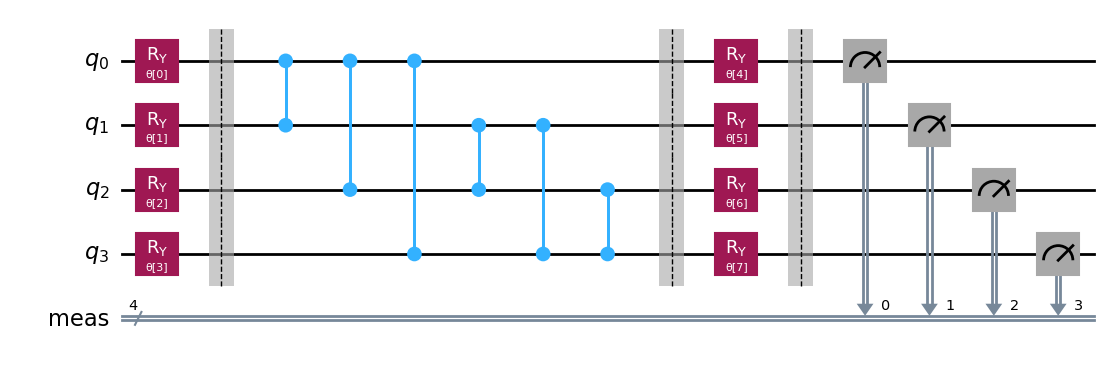
\includegraphics[width=0.8\textwidth]{images/circuitoVQE.png}
    \caption{Circuito parametrizzato per il VQE, generato con l'ansatz \texttt{TwoLocal}.}
    \label{fig:vqe_circuit}
\end{figure}

Un esempio di risultato di un'esecuzione del VQE è mostrato nella Figura~\ref{fig:risultatoVQE}, 
in cui si evidenziano la configurazione ottimale degli asset e il valore della 
funzione obiettivo. Questo risultato rappresenta l'allocazione di portafoglio 
ottimale secondo il modello definito.



\paragraph{Risoluzione con QAOA}
Un secondo approccio che abbiamo deciso di utilizzare per risolvere il problema del PO 
è stato quello del QAOA. Come descritto nella Sezione~\ref{sec:qaoa}, questo algoritmo 
utilizza un'architettura parametrizzata che integra circuiti quantistici e ottimizzatori 
classici, con l'obiettivo di approssimare la configurazione ottimale attraverso un 
processo iterativo di adattamento dei parametri.

In una prima fase, abbiamo provato a implementare manualmente il QAOA, ma questa 
soluzione si è rivelata poco efficiente dal punto di vista computazionale, richiedendo 
tempi di esecuzione eccessivamente lunghi. Per una questione di ottimizzazione e 
scalabilità, è stato quindi deciso di utilizzare la classe \texttt{QAOA} offerta da 
Qiskit~\cite{qiskit_portfolio_optimization}, che fornisce un'implementazione già ottimizzata dell'algoritmo.

Il circuito parametrizzato del QAOA è stato configurato con il numero di ripetizioni 
(\texttt{reps=1}) e l'ottimizzatore COBYLA per la ricerca dei parametri ottimali. 
Il codice per configurare e risolvere il problema è il seguente:

\begin{lstlisting}[language=python]
 qaoa_mes = QAOA(sampler=Sampler(), optimizer=cobyla, reps=1)
 qaoa = MinimumEigenOptimizer(qaoa_mes, penalty)
 result_qaoa = qaoa.solve(qp)
\end{lstlisting}

La Figura~\ref{fig:qaoa_circuit} mostra lo schema del circuito generato, evidenziando 
i layer parametrizzati e le connessioni tra i qubit.

\begin{figure}[h!]
    \centering
    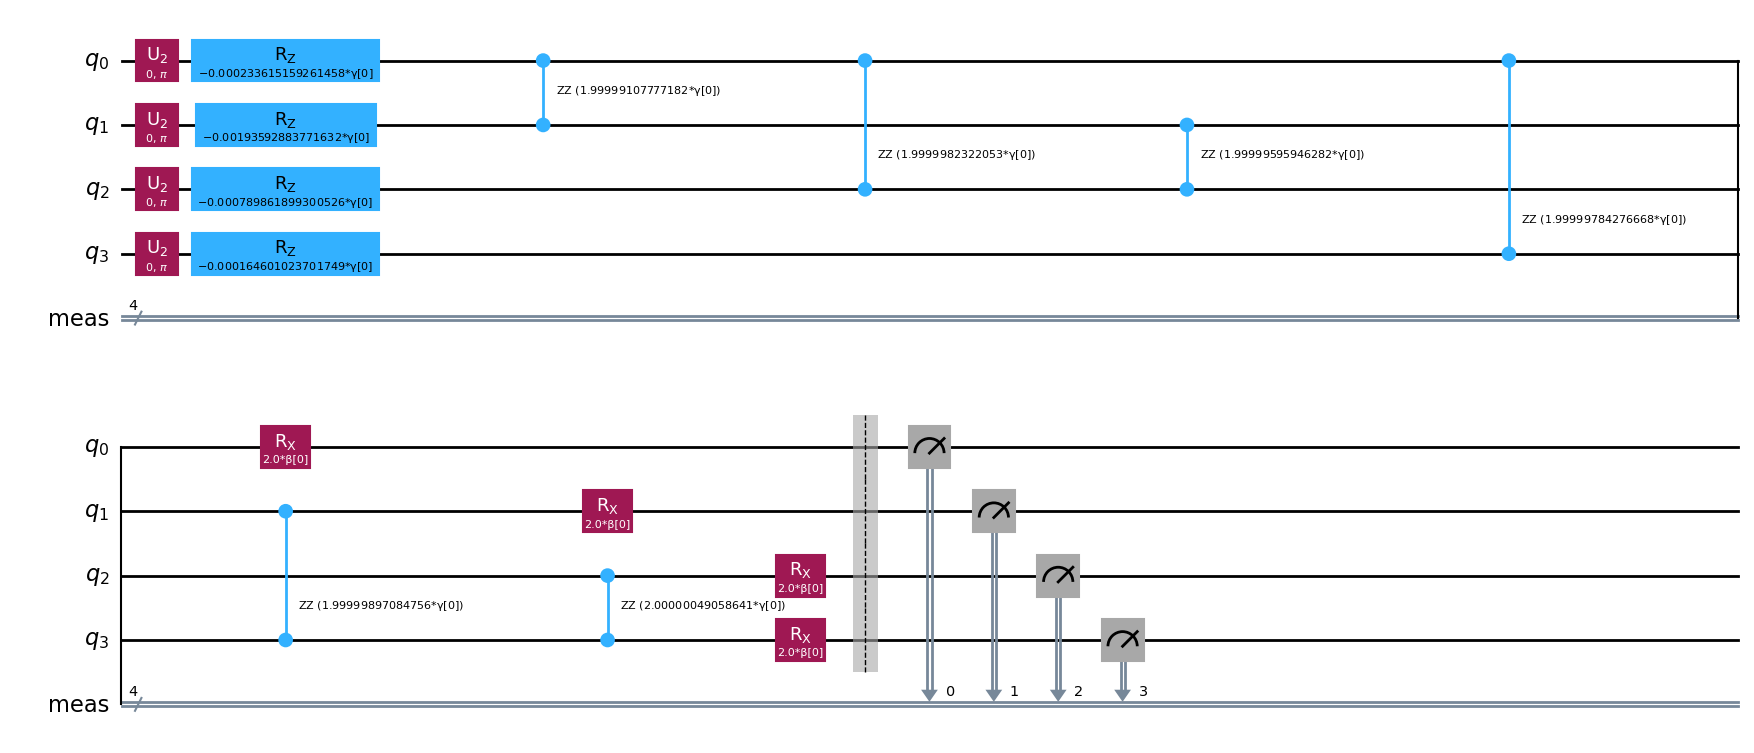
\includegraphics[width=0.8\textwidth]{images/circuitoQAOA.png}
    \caption{Circuito parametrizzato per il QAOA.}
    \label{fig:qaoa_circuit}
\end{figure}

Un esempio di risultato di un'esecuzione del QAOA è mostrato nella 
Figura~\ref{fig:risultatoQAOA}, che evidenzia la configurazione ottimale degli asset 
e il valore della funzione obiettivo.



\subsection{Introduzione del rumore}

Finora, gli algoritmi VQE e QAOA sono stati simulati assumendo un sistema ideale, 
privo di rumore. Tuttavia, per avvicinare l'implementazione alla realtà dei computer 
quantistici attuali, abbiamo introdotto un modello di rumore basato su un backend 
generico, \texttt{GenericBackendV2}, offerto da Qiskit. Questo backend consente 
di configurare simulazioni personalizzate, adattandosi al numero di qubit richiesti 
e fornendo dettagli sul rumore associato al dispositivo simulato.

Il modello di rumore è stato generato utilizzando la classe \texttt{NoiseModel} 
e applicato al simulatore quantistico \texttt{AerSimulator}:

\begin{lstlisting}[language=python, caption={Configurazione del modello di rumore per la simulazione.}]
 # Configurazione del backend generico
 backend = GenericBackendV2(
     num_qubits=assets, 
     noise_info=True,
     seed=seed,
     calibrate_instructions=True
 )
 
 # ...
 
 # Generazione del modello di rumore
 noise_model = NoiseModel.from_backend(backend)
 simulator = AerSimulator(noise_model=noise_model)
\end{lstlisting}

Il backend \texttt{GenericBackendV2} è stato configurato per adattarsi al numero 
di qubit utilizzati nel problema di ottimizzazione del portafoglio (\texttt{assets}). 
L'opzione \texttt{noise\_info} è stata abilitata per includere dettagli realistici 
sulle fonti di rumore, mentre la calibrazione automatica delle istruzioni 
(\texttt{calibrate\_instructions=True}) garantisce una maggiore fedeltà nella 
simulazione del comportamento del dispositivo.

Il modello di rumore generato include informazioni relative ad errori di decoerenza, 
errori di misura e altre imperfezioni che caratterizzano i computer quantistici 
attuali. Più nel dettaglio, è stato implementato un modello che include un errore 
di flip del 5\%, un errore di depolarizzazione dell'1\% per gate a 1 qubit e del 2\%
per gate a 2 qubit, e un errore del 2\% sulle misure. Questa configurazione ha 
permesso di valutare le prestazioni degli algoritmi in un contesto più realistico 
rispetto a un sistema ideale, dove ci aspettiamo un moderato deterioramento delle 
prestazioni.


%%%%%%%%%%%%%%%%%%%%%%%%%%%%%%%%%%%% VQE noisy %%%%%%%%%%%%%%%%%%%%%%%%%%%%%%%%%%%%%

\paragraph{Implementazione del VQE con rumore} 

Per il VQE con rumore, è stato utilizzato lo stesso circuito usato nella versione senza rumore.

\begin{lstlisting}[language=python, caption={Configurazione dell'ansatz per il VQE.}]
 ansatz = TwoLocal(
     num_qubits=assets,
     rotation_blocks="ry",
     entanglement_blocks="cz",
     reps=1,
     entanglement="full",
     insert_barriers=True
 )
\end{lstlisting}

Successivamente, l'ansatz è stato decomposto per ottenere una rappresentazione più 
dettagliata del circuito e adattato al backend rumoroso tramite la transpilazione.

\begin{lstlisting}[language=python, caption={Decomposizione e transpilazione dell'ansatz per il backend rumoroso.}]
 decomposed_ansatz = ansatz.decompose()
 transpiled_ansatz = transpile(decomposed_ansatz, 
                               backend=backend)
\end{lstlisting}

Il circuito transpiled è stato poi utilizzato per configurare il metodo \texttt{SamplingVQE}, 
combinato con l'ottimizzatore COBYLA per minimizzare l'energia del sistema.

\begin{lstlisting}[language=python, caption={Configurazione e risoluzione del VQE con rumore.}]
 svqe_mes_noisy = SamplingVQE(sampler=Sampler(), 
                              ansatz=transpiled_ansatz, 
                              optimizer=cobyla)
 svqe_noisy = MinimumEigenOptimizer(svqe_mes_noisy, penalty)
 result_svqe_noisy = svqe_noisy.solve(qp)
\end{lstlisting}

La Figura~\ref{fig:vqe_noisy_circuit} mostra il circuito utilizzato per il VQE con rumore.

\begin{figure}[h!]
    \centering
    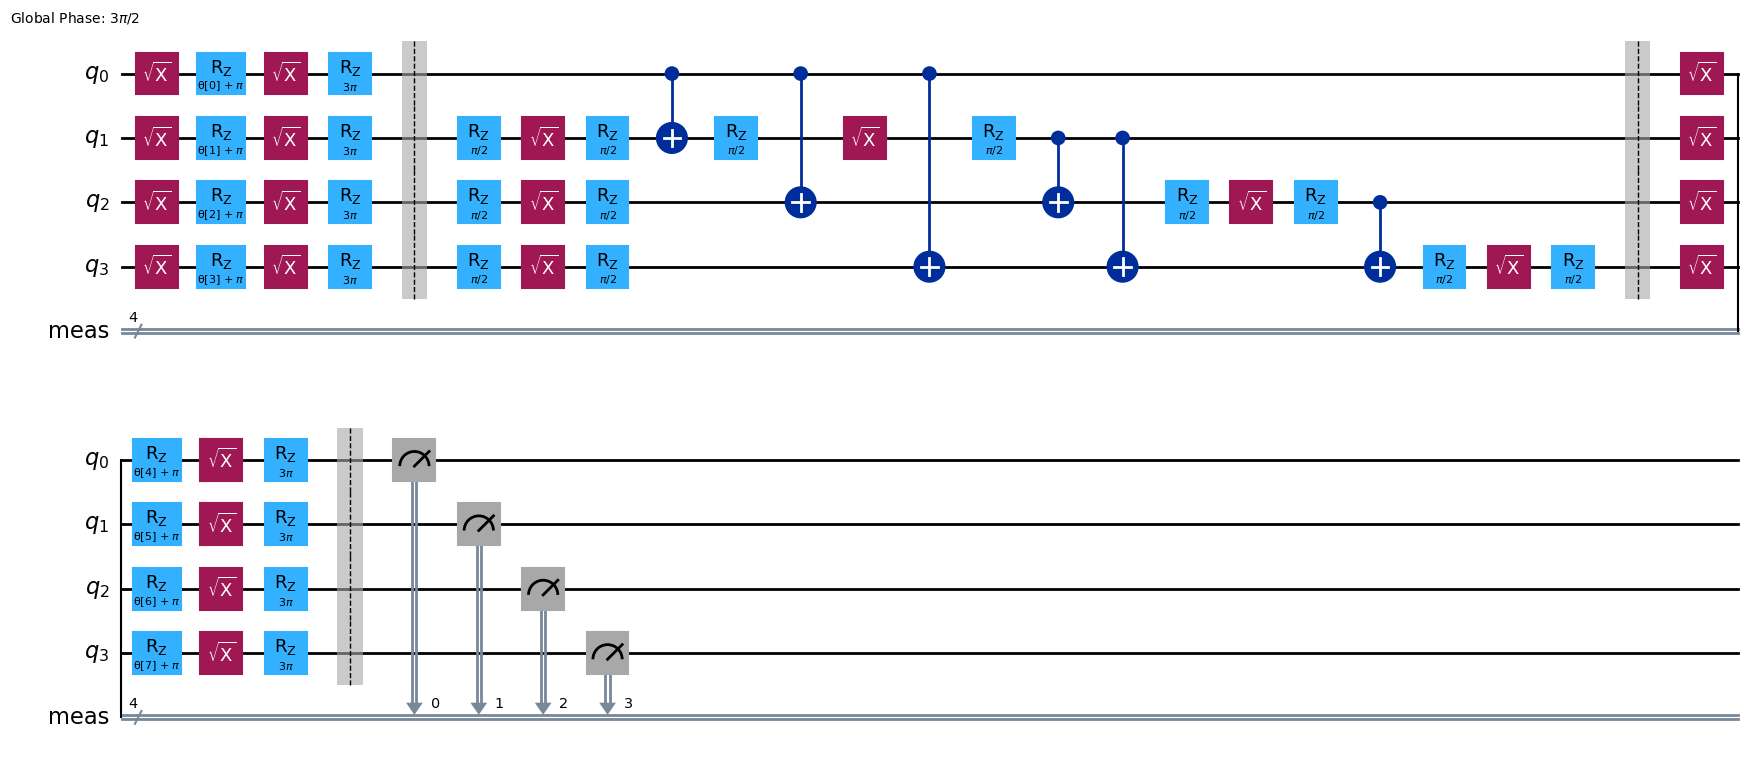
\includegraphics[width=0.8\textwidth]{images/circuitoVQEnoisy.png}
    \caption{Circuito a 4 qubit parametrizzato per il VQE con rumore.}
    \label{fig:vqe_noisy_circuit}
\end{figure}



%%%%%%%%%%%%%%%%%%%%%%%%%%%%%%%%%%%% QAOA noisy %%%%%%%%%%%%%%%%%%%%%%%%%%%%%%%%%%%%%

\paragraph{Implementazione del QAOA con rumore}

Anche il QAOA è stato implementato tenendo conto del rumore simulato tramite il backend 
\texttt{GenericBackendV2}. Come per il VQE, il circuito parametrizzato è stato adattato 
al backend rumoroso per rappresentare fedelmente le caratteristiche di un computer 
quantistico reale.

L'algoritmo è stato inizialmente configurato con la classe \texttt{QAOA}, utilizzando 
il sampler \texttt{Sampler()} e l'ottimizzatore COBYLA. Una prima esecuzione del 
metodo \texttt{solve} è stata necessaria per generare automaticamente il circuito 
iniziale, successivamente decomposto e transpiled per adattarsi al backend rumoroso. 
Con il circuito adattato, una seconda esecuzione del metodo \texttt{solve} ha 
permesso di risolvere il problema di ottimizzazione. 
Il codice completo è mostrato di seguito.

\begin{lstlisting}[language=python, caption={Implementazione del QAOA con rumore.}]
 # Configurazione e prima esecuzione del QAOA
 qaoa_mes_noisy = QAOA(sampler=Sampler(), optimizer=cobyla, reps=1)
 qaoa_noisy = MinimumEigenOptimizer(qaoa_mes_noisy, penalty)
 _ = qaoa_noisy.solve(qp)

 # Decomposizione e transpilazione del circuito
 decomposed_circuit_noisy = qaoa_mes_noisy.ansatz.decompose()
 transpiled_circuit_noisy = transpile(decomposed_circuit_noisy, backend=backend)
 qaoa_mes_noisy.ansatz = transpiled_circuit_noisy

 # Risoluzione finale del QAOA
 result_decomposed = qaoa_noisy.solve(qp)
\end{lstlisting}

La Figura~\ref{fig:qaoa_noisy_circuit} mostra il circuito transpiled utilizzato 
per il QAOA con rumore.

\begin{figure}[h!]
    \centering
    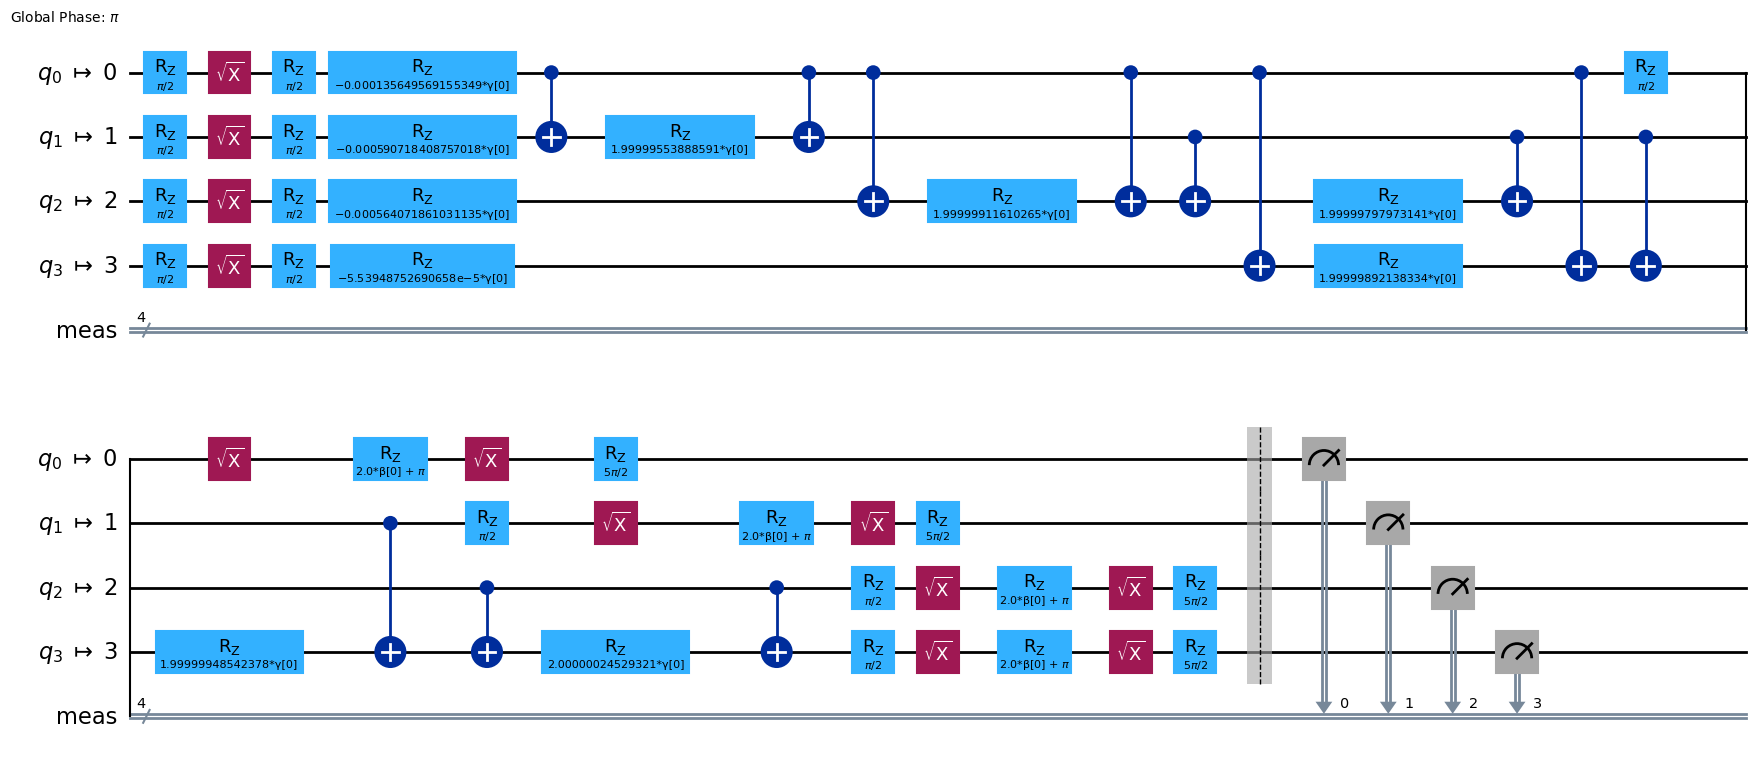
\includegraphics[width=0.8\textwidth]{images/circuitoQAOAnoisy.png}
    \caption{Circuito a 4 qubit parametrizzato per il QAOA con rumore.}
    \label{fig:qaoa_noisy_circuit}
\end{figure}





\begin{figure}[h!]
    \centering
    \begin{subfigure}{0.49\textwidth}
        \centering
        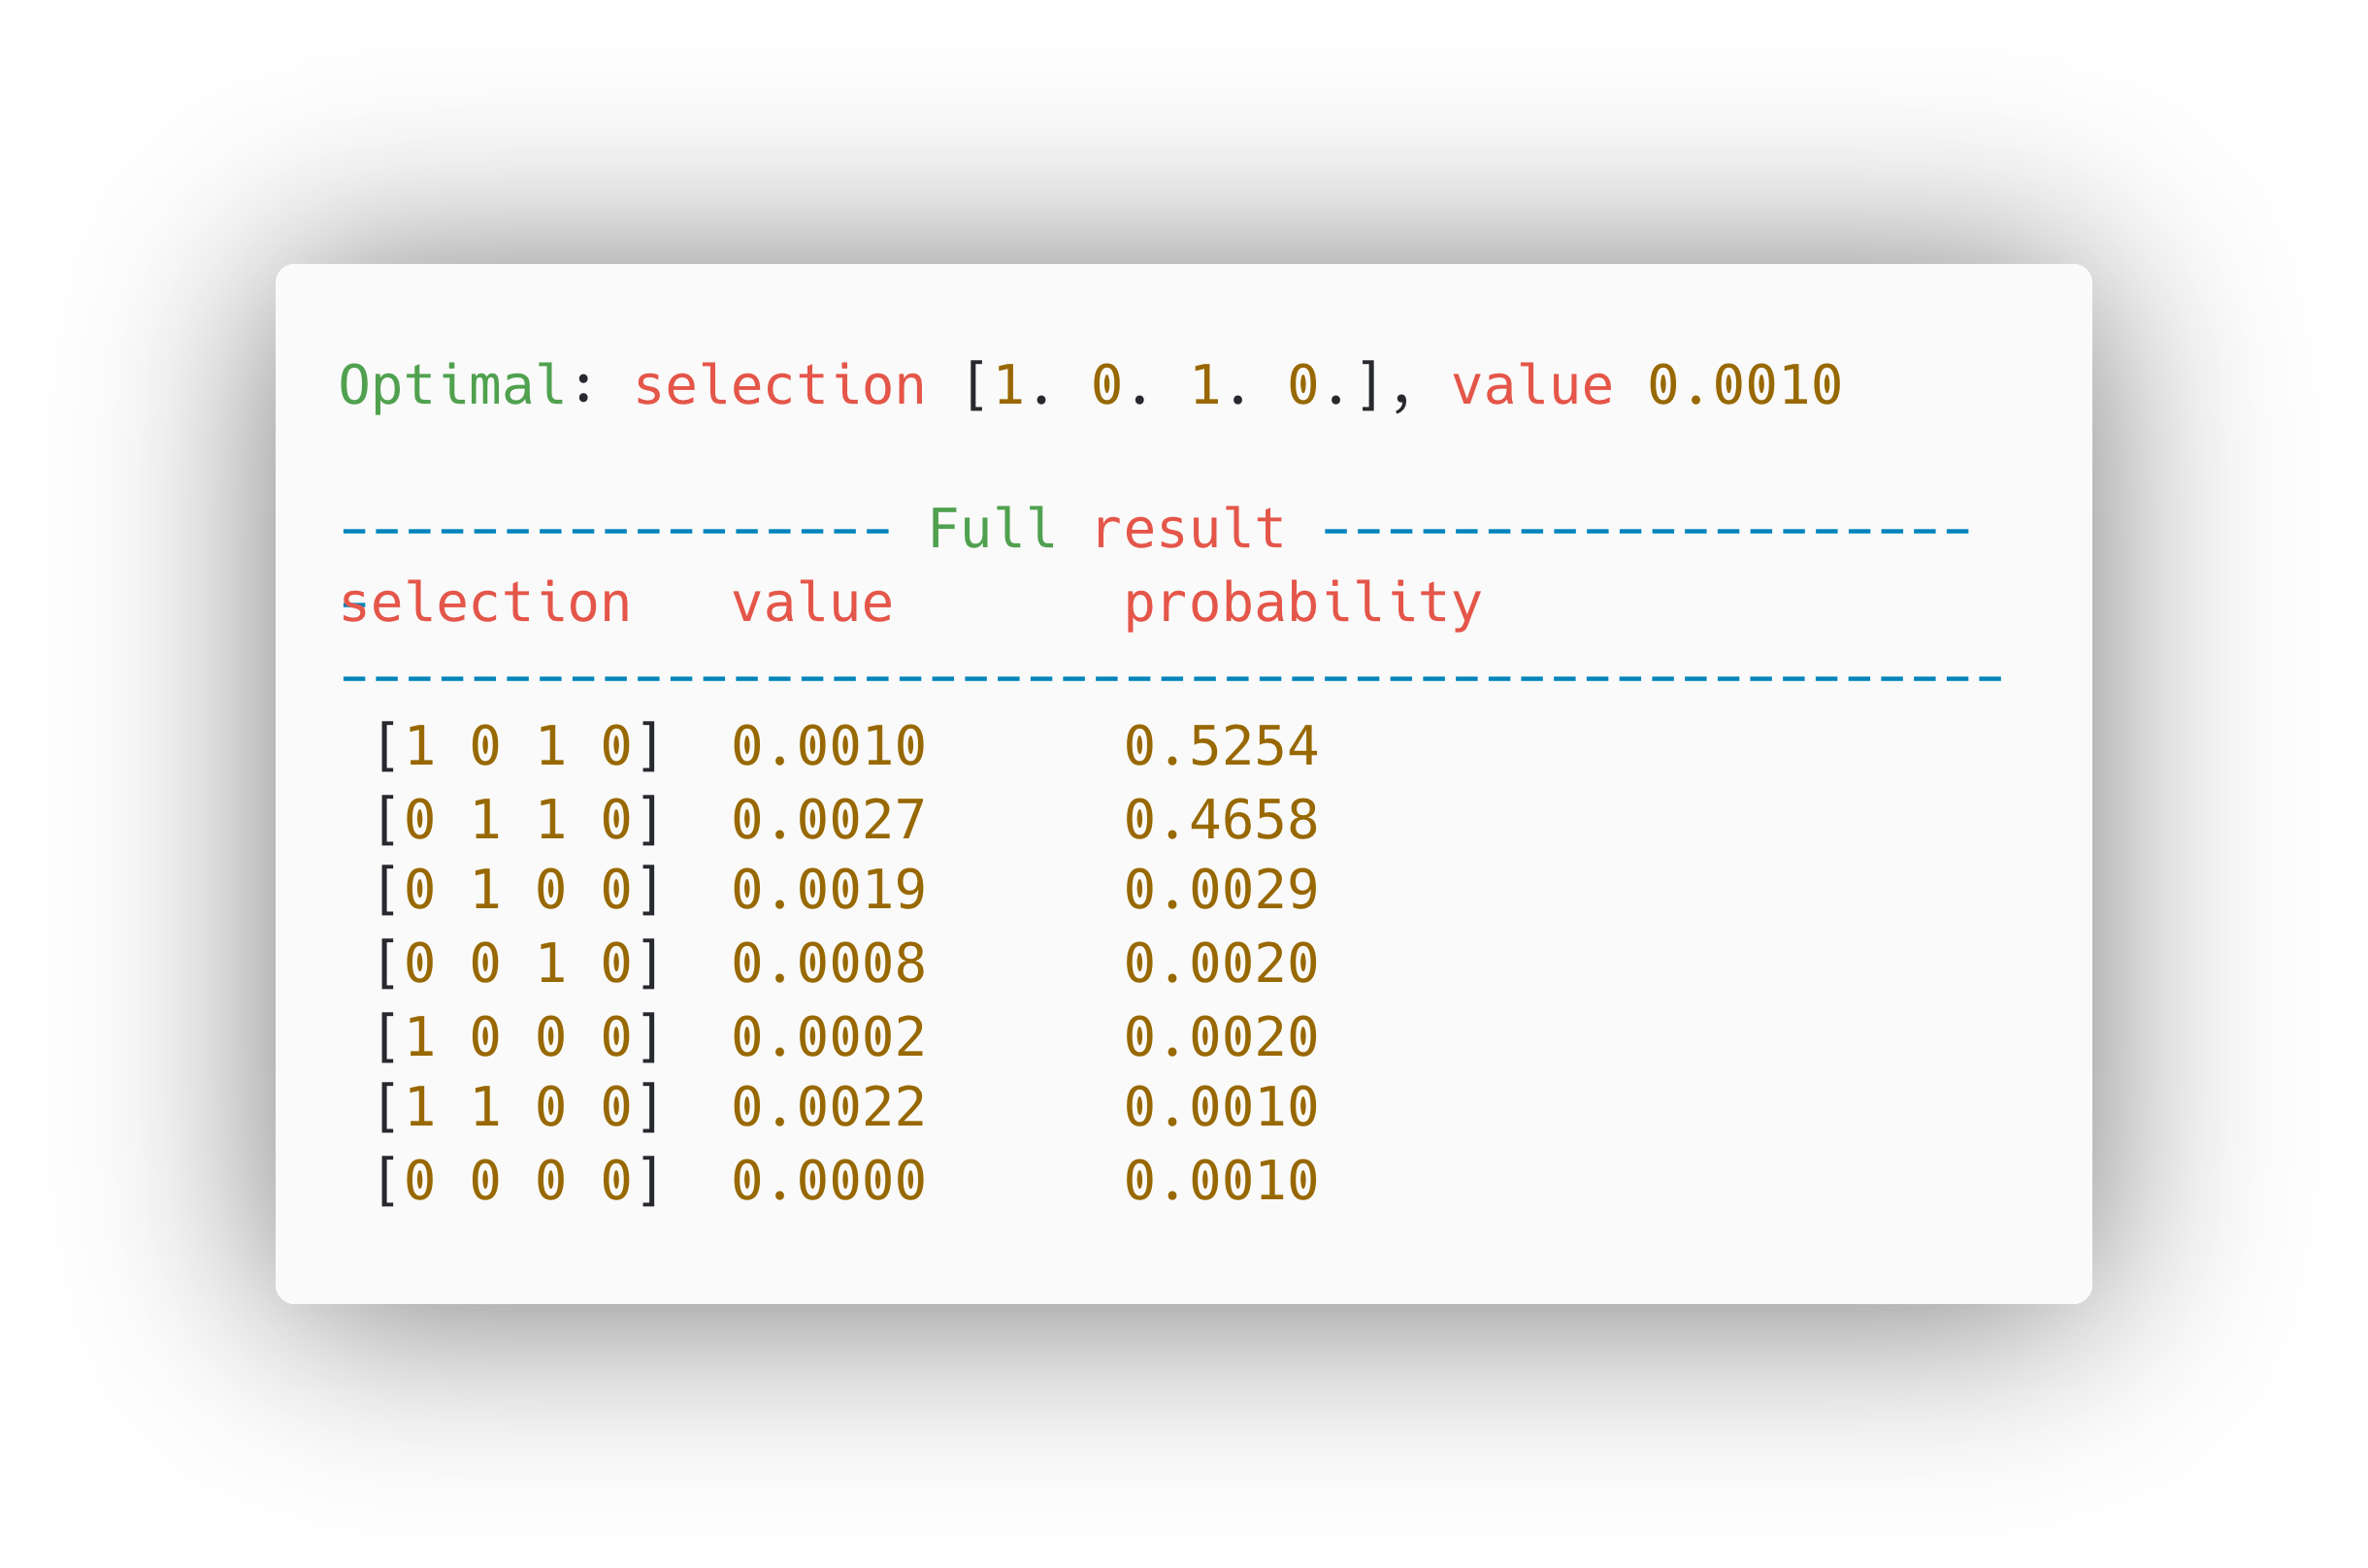
\includegraphics[width=\textwidth]{images/risultatoVQE.png}
        \caption{Risultato ottenuto con VQE.}
        \label{fig:risultatoVQE}
    \end{subfigure}
    \hfill
    \begin{subfigure}{0.49\textwidth}
        \centering
        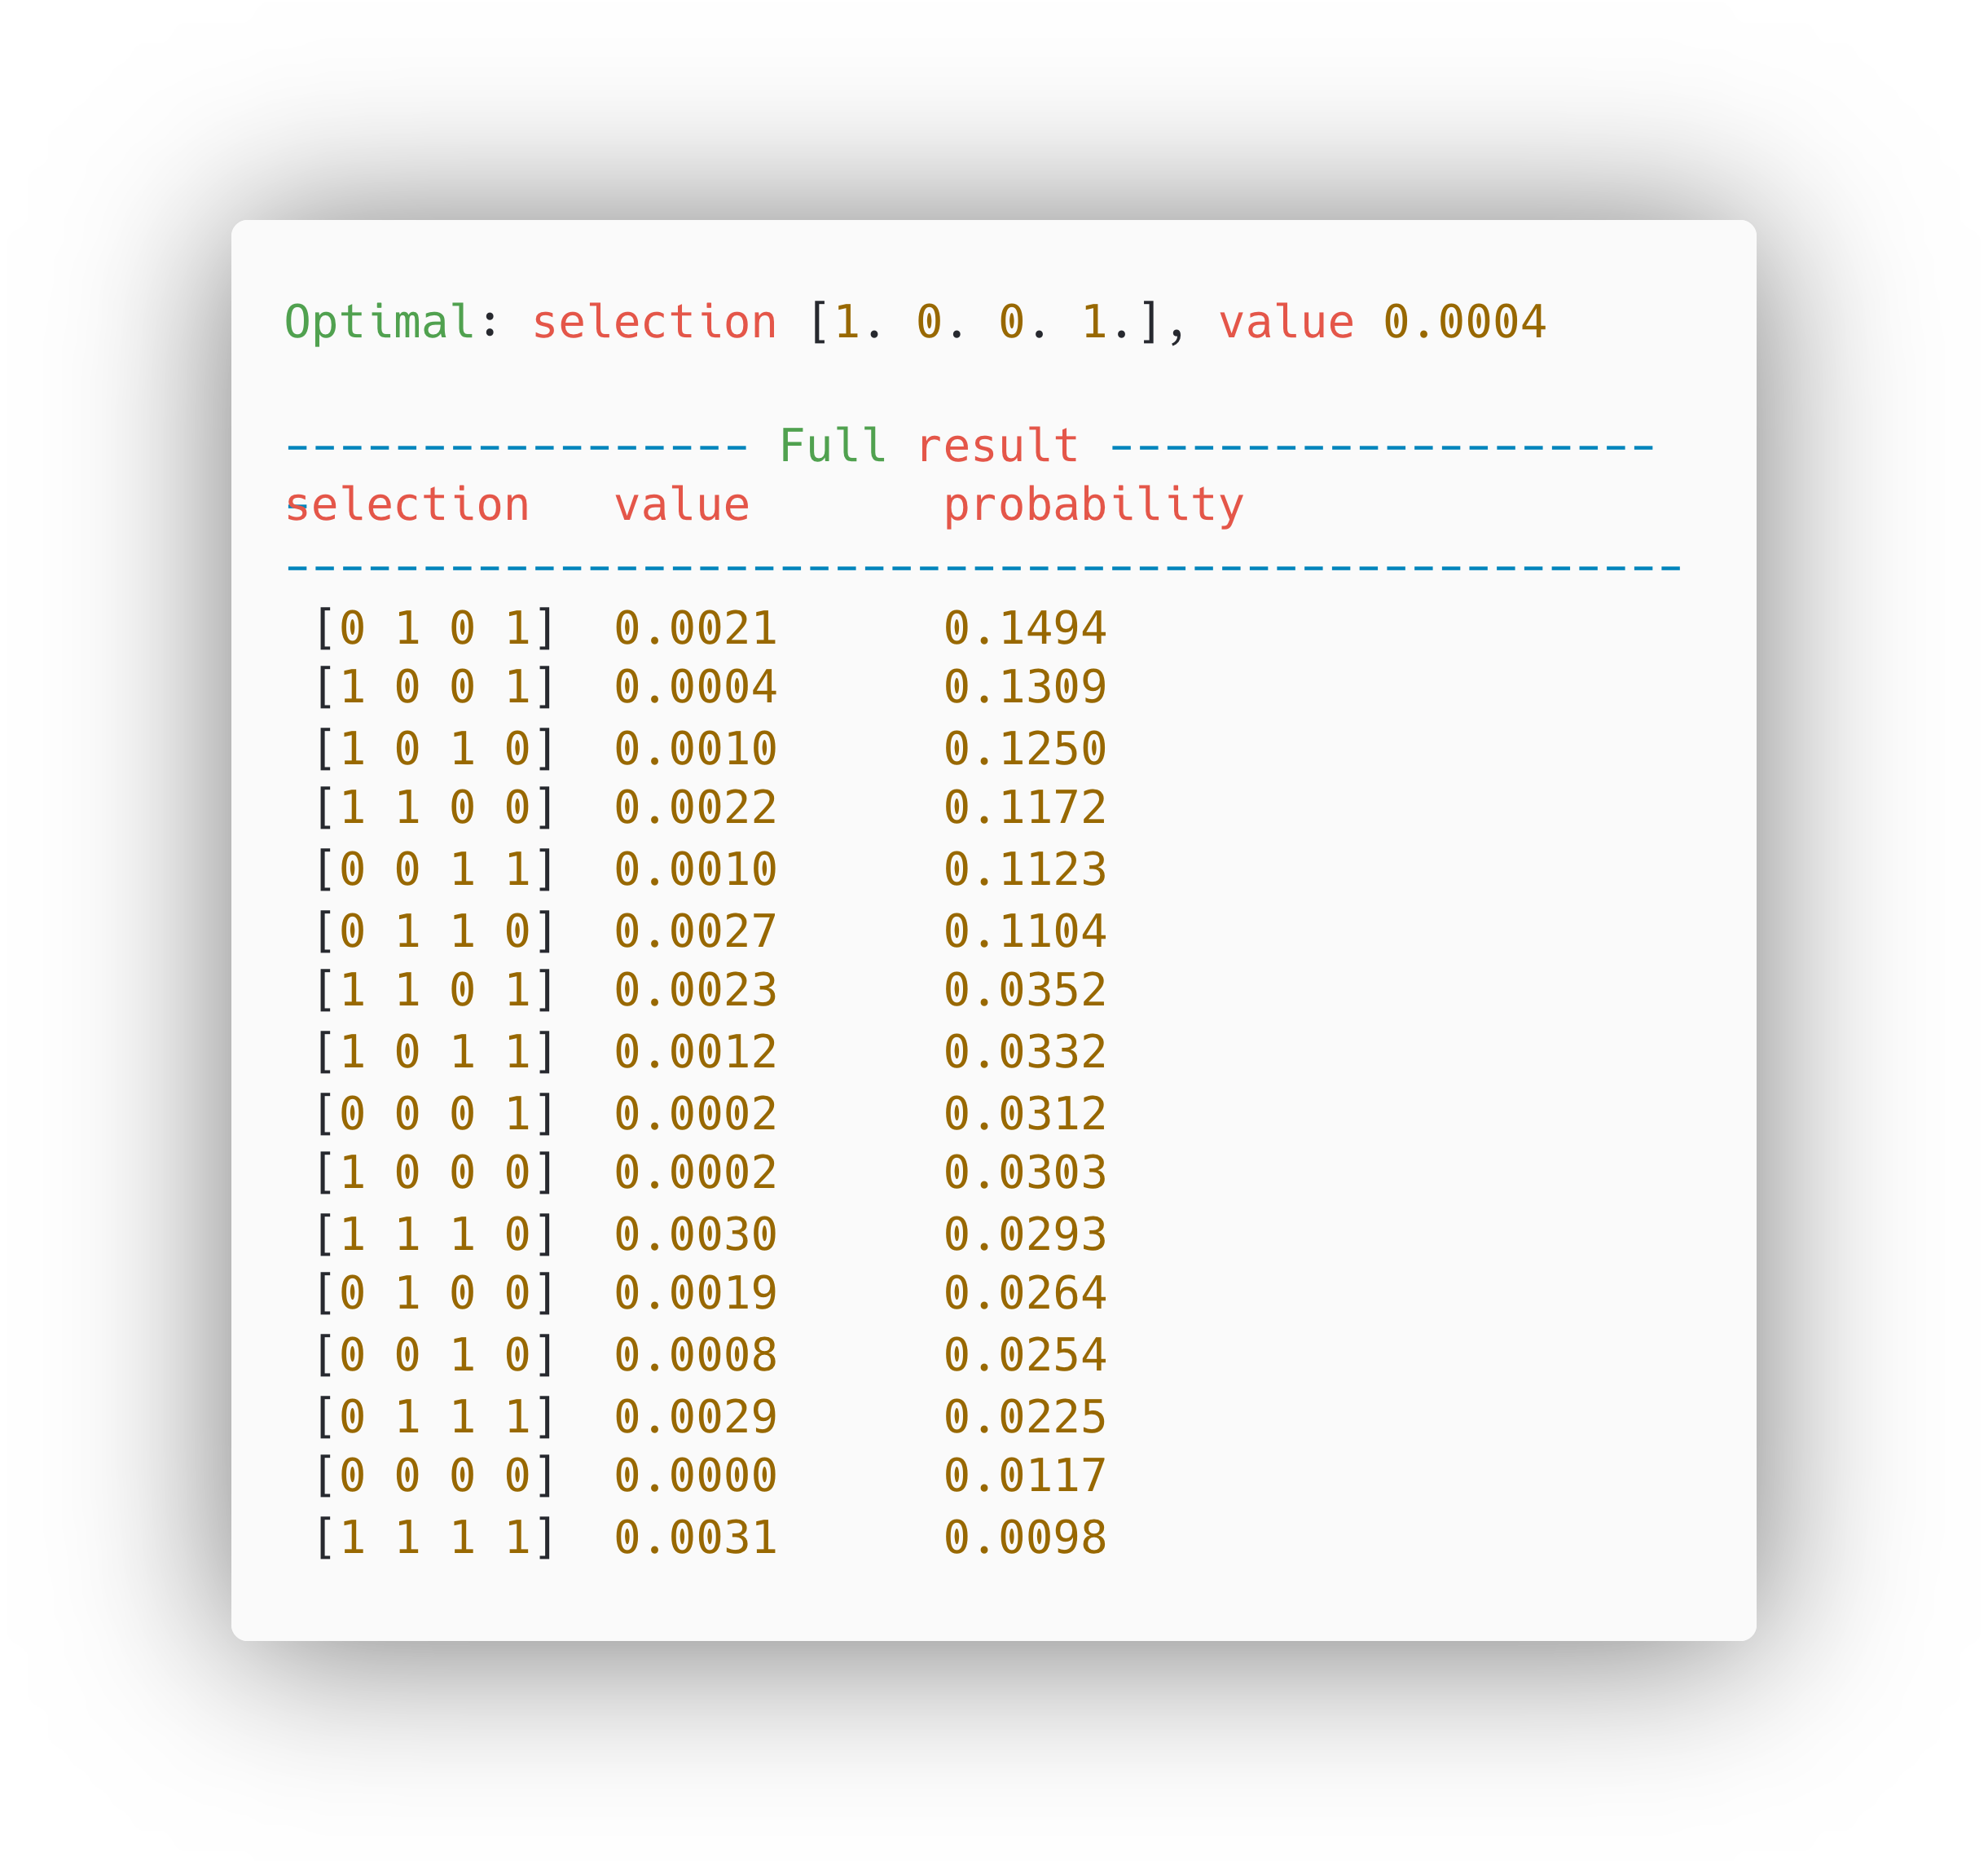
\includegraphics[width=\textwidth]{images/risultatoQAOA.png}
        \caption{Risultato ottenuto con QAOA.}
        \label{fig:risultatoQAOA}
    \end{subfigure}
    \hfill
    \begin{subfigure}{0.60\textwidth}
        \centering
        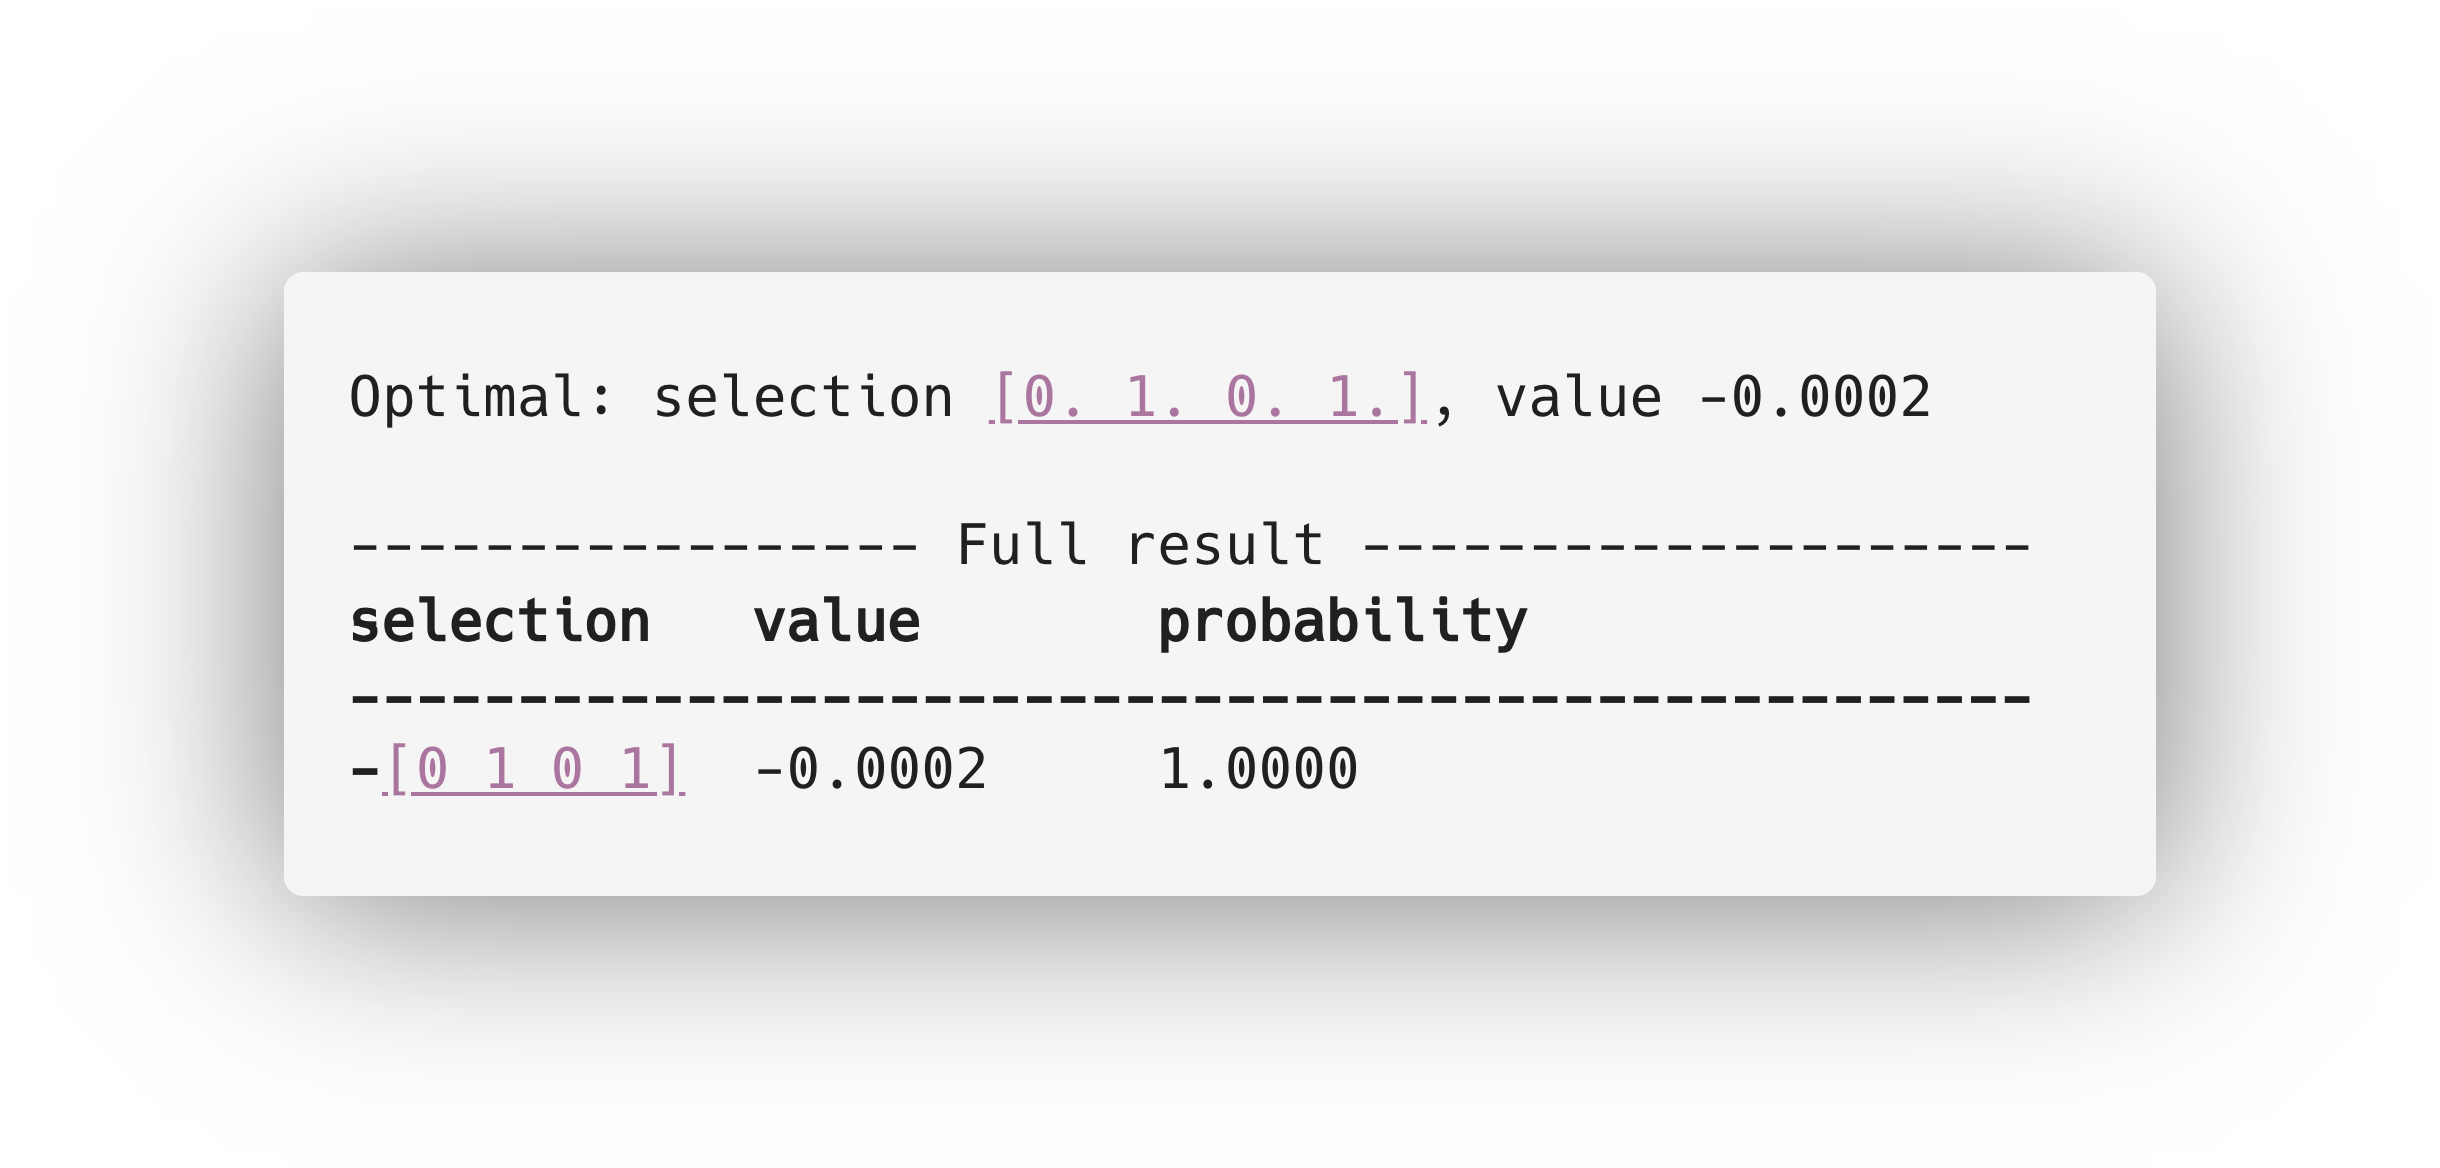
\includegraphics[width=\textwidth]{images/risultatoClassico.png}
        \caption{Risultato ottenuto con il risolutore classico.}
        \label{fig:risultatoClassico}
    \end{subfigure}
    \caption{Risultati ottenuti con (a) VQE, (b) QAOA e (c) risolutore classico.}
    %\label{fig:}
\end{figure}